\let\negmedspace\undefined
\let\negthickspace\undefined
\documentclass[journal]{IEEEtran}
\usepackage[a5paper, margin=10mm, onecolumn]{geometry}
%\usepackage{lmodern} % Ensure lmodern is loaded for pdflatex
\usepackage{tfrupee} % Include tfrupee package

\setlength{\headheight}{1cm} % Set the height of the header box
\setlength{\headsep}{0mm}  % Set the distance between the header box and the top of the text

\usepackage{gvv-book}
\usepackage{gvv}
\usepackage{cite}
\usepackage{amsmath,amssymb,amsfonts,amsthm}
\usepackage{algorithmic}
\usepackage{graphicx}
\usepackage{textcomp}
\usepackage{xcolor}
\usepackage{txfonts}
\usepackage{listings}
\usepackage{enumitem}
\usepackage{mathtools}
\usepackage{gensymb}
\usepackage{comment}
\usepackage[breaklinks=true]{hyperref}
\usepackage{tkz-euclide} 
\usepackage{listings}
% \usepackage{gvv}                                        
\def\inputGnumericTable{}                                 
\usepackage[latin1]{inputenc}                                
\usepackage{color}                                            
\usepackage{array}                                            
\usepackage{longtable}                                       
\usepackage{calc}                                             
\usepackage{multirow}                                         
\usepackage{hhline}                                           
\usepackage{ifthen}                                           
\usepackage{lscape}

% Marks the beginning of the document
\begin{document} 

\bibliographystyle{IEEEtran}
\vspace{3cm}

\title{1-1.5-8}
\author{EE24BTECH11029- JANAGANI SHRETHAN REDDY}
\maketitle
\bigskip
\renewcommand{\thefigure}{\theenumi}
\renewcommand{\thetable}{\theenumi}

Question$\colon$
     Find the ratio in which $P\brak{4,5}$ divides the line segment joining $A\brak{2,3}$ and $B\brak{7,8}$\\

solution $\colon$
\begin{table}[h!]
 \centering
 \begin{tabular}{|c|c|c|}
\hline
variable& Description&formula
\\\hline
\multirow{3}{1em}\\A$\brak{2,3}$&one end of the line segment&$-$
\\\hline
B$\brak{7,8}$&another end of the line segment&$-$
\\\hline
P $\brak{4,5}$&divides$\vec{A}$and $\vec{B}$ in the ratio $k\colon1$&$ P=\frac{\vec{A}+k\vec{B}}{k+1}$
\\\hline
\end{tabular}

 \caption{variable used}
\end{table}\\
 $P\myvec{4&5}$ divides $A$ and $B$ in the ratio $k\colon1$
\begin{align}
 P&=\frac{\vec{A}}{k+1}+\frac{k\vec{B}}{k+1}\\
\implies p&=\myvec{\Vec{A}&\Vec{B}}\myvec{\frac{1}{k+1}\\\frac{k}{k+1}}\\
\implies \myvec{4\\5}&=\myvec{2&7\\3&8}\myvec{\frac{1}{k+1}\\\frac{k}{k+1}}\\
\implies \myvec{4\\5}&=\myvec{\frac{2}{k+1}+\frac{7k}{k+1}\\\frac{3}{k+1}+\frac{8k}{k+1}}\\
\implies 4&=\frac{2+7k}{k+1}\\
\implies 4k+4&=2+7k\\
3k&=2\\
k&=\frac{2}{3}\\
\implies k\colon1&=\frac{2}{3}\colon1
 \end{align}
 \begin{figure}[h!]
  \centering
  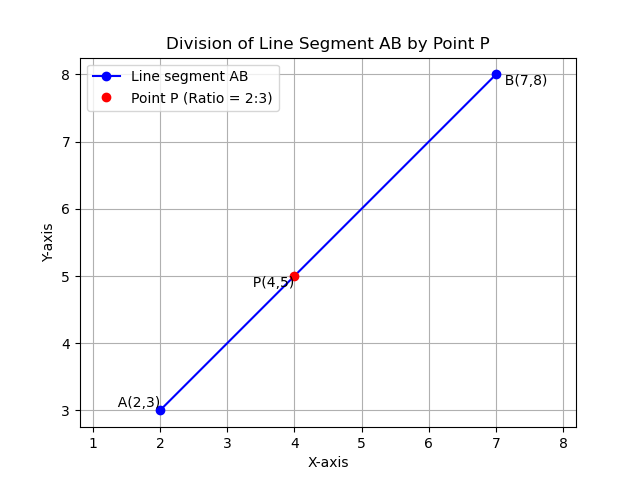
\includegraphics[width=1\linewidth]{fig.png}
  \caption{plot of A,B and P}
 \end{figure}
 
\end{document}
